%\vspace{-0.12in}
\chapter{App Dependency Analyzer}
\label{sec:depedency}
\begin{comment}
{
\section{Overview}
Each smart app can subscribe to events generated by one or more devices. In each subscription, the smart app provides a call back function (\textit{i.e.}, event handler) to SmartThings. Upon the occurrence of the subscribed event, SmartThings will trigger the registered event handler. Moreover, SmartThings also allows apps to register call back functions that will be triggered at some scheduled time. In summary, each smart app may have one or more event handlers. \textit{App Dependency Analysis} takes a set of event handlers of apps as inputs, build a dependency graph (DG), and calculating dependent sets. The event handlers in each dependent set need to be verified together since the inter-action among them may result in some violations. Moreover, the event handlers in different dependent sets may have conflicting behaviors, which may result in conflicting command violation. Therefore, the event handlers involving in a conflict also needs to be verified together.
}
\end{comment}

\begin{table}[bt]
\scriptsize
\ssp
\caption{An example to showcase the construction of a dependency graph.}
%\vspace{-0.12in}
\label{dgconstructiontb}
\centering
\begin{tabular}{| p{2.7cm} | l | p{1.5cm} | p{2.6cm} | p{2.5cm} |}
\hline
\bf App's Name & \bf Event Handler & \bf Vertex's ID & \bf Input Events & \bf Output Events\\
\hline
Brighten Dark Places & contactOpenHandler & 0 & contact/open, illuminance/``..." &  switch/on\\
\hline
Let There Be Dark! & contactHandler & 1 & contact/``..." &  switch/on, switch/off\\
\hline
Auto Mode Change & presenceHandler & 2 & presence/``..." &  location/mode\\
\hline
\multirow{2}{2.7cm}{Unlock Door}  & appTouch & 3 & app/touch & lock/unlocked\\ \cline{2-5}
	& changedLocationMode & 4 & location/mode & lock/unlocked\\
\hline
\multirow{2}{3cm}{Big Turn On}  & appTouch & 5 & app/touch & switch/on\\ \cline{2-5}
	& changedLocationMode & 6 & location/mode & switch/on\\
\hline
\end{tabular}
%\vspace{-0.13in}
\end{table}

%The first module of \sys determines sets of apps that are inter-dependent \textit{i.e.}, can jointly influence
%actuator actions. The reason for doing this is that,

The model checker should not have to check the interactions
between event handlers that do not interact. To find
event handlers that can interact and thus jointly influence actuator actions,
this module constructs a {\em dependency graph} (DG).
%This graph consists of
%{\em dependent sets} of apps \textit{i.e.}, sets of apps that interact either directly or indirectly.

\begin{comment}
{
\begin{figure}[t]
\begin{center}
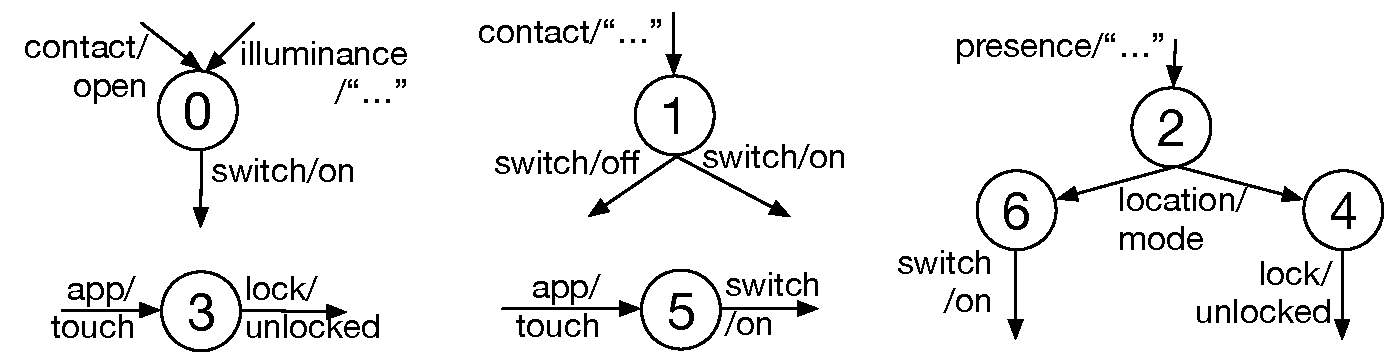
\includegraphics[width=3.0in]{DependencyGraphExample}
\vspace{-0.13in}
\caption{Example of a dependency graph.}
\label{dgconstructionfg}
\end{center}
\vspace{-0.33in}
\end{figure}
}
\end{comment}

\begin{figure}[bt]
    \centering
    \begin{subfigure}[t]{3.5in}
        \centering
        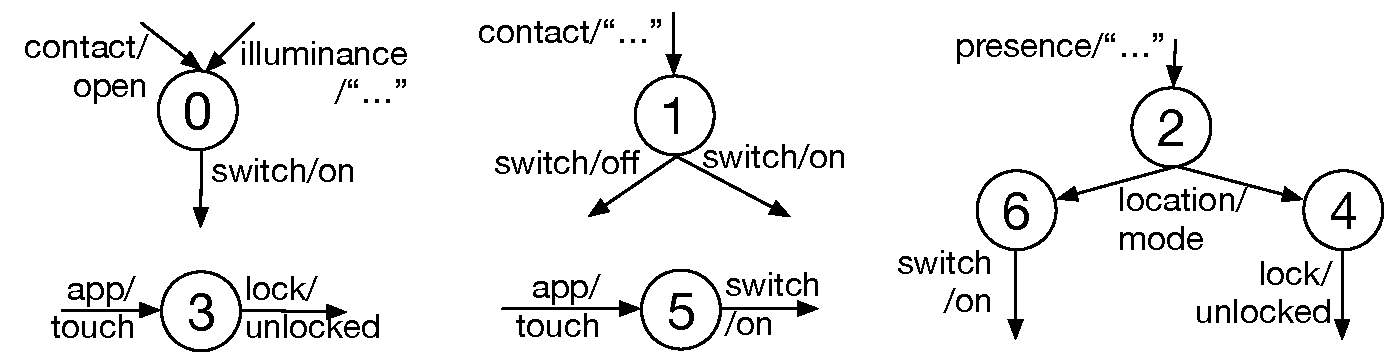
\includegraphics[width=3.5in]{DependencyGraphExample}
				%\vspace{-0.22in}
		\caption{Dependency graph.}
        \label{dgconstructionfg}
    \end{subfigure}\\
    \vspace{0.05in}
    \begin{subfigure}[t]{3.3in}
        \centering
        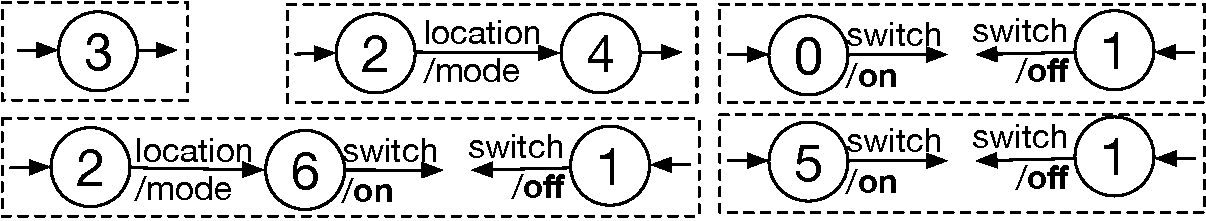
\includegraphics[width=3.3in]{related_set}
				%\vspace{-0.22in}
        \caption{\textcolor{black}{Related sets (each box represents a related set).}}
		%\vspace{-0.15in}
        \label{relatedset}
    \end{subfigure}
    \caption{Example of a dependency graph and its corresponding related sets.}
%\vspace{-0.25in}
\end{figure}

\section{Extracting Input/Output Events}
{\color{black}Each smart app registers one or more {\em event handlers} that get notified of events to
which it has subscribed.
%\zhiyun{each smart app has only one callback function? If so, maybe we should just say each vertex is an app to be more clear.}\thomas{No, one app may have several callback functions.}
An event handler takes one or more input events, and can induce zero or more output events.
Input events are (i) explicitly declared in the \texttt{subscribe} commands or,
(ii) identified via APIs that read states of smart devices,
or (iii) indicated by interrupts at specific times defined by \texttt{schedule} method calls.
Output events are invoked via APIs that change states of smart devices.

{\color{black}We enumerate the input and output events of an app using static analysis
%(details are straightforward and are omitted to save space).}
as follows. First, we parse and identify
all the read and write APIs in each function of the smart app. Second, we build call sequences whose entry points are event handlers. The input events of an event handler are identified by (i) the read APIs in its call sequence, (ii)
the events specified in its \textit{subscribe}, and times in its \textit{schedule} method calls.
The output events are identified by the write APIs in its call sequence.}

\section{Dependency Graph Construction}
\begin{comment}
Each smart app registers one or more {\em event handlers} that get notified of events to
which it has subscribed.
%\zhiyun{each smart app has only one callback function? If so, maybe we should just say each vertex is an app to be more clear.}\thomas{No, one app may have several callback functions.}
An event handler takes one or more input events, and can induce zero or more output events.
Input events are (i) explicitly declared in the \texttt{subscribe} commands or,
(ii) identified via APIs that read states of smart devices,
or (iii) indicated by interrupts at specific times defined by \texttt{schedule} method calls.
Output events are invoked via APIs and change states of smart devices.
We enumerate the input and output events of an app using static analysis
(details are straightforward thus omitted due to space constraints).
%as follows. First, we parse and identify
%all the read and write APIs in each function of the smart app. Second, we build call sequences whose entry points are event handlers. The input events of an event handler are identified by (i) the read APIs in its call sequence, (ii)
%the events specified in its \textit{subscribe}, and times in its \textit{schedule} method calls.
%The output events are identified by the write APIs in its call sequence.
\end{comment}
Once the input and output events are identified,
we construct a directed DG as follows.
Each event handler is denoted by a vertex in the DG.
An edge from a vertex $u$ to a vertex $v$ ($u \rightarrow v$) is added
if the output events of $u$ overlap with the input events of $v$.
$u$ is then called the \textit{parent} vertex of the \textit{child} vertex $v$.
The vertices in a strongly connected component are merged into a composite vertex (a union of input and output events).
A \textit{leaf} vertex does not have any child.

\section{Example}
To illustrate, consider the following example.
Table~\ref{dgconstructiontb} summarizes the event handlers and the associated input/output
events with a set of sample smart apps.
The description of an event is in the format \textit{attribute}/\textit{event type}
(\eg, contact/open means ``a contact sensor is open");
empty quotes (``...") denote ``any" event of that type.
Given these apps, we show the DG that is built in Figure~\ref{dgconstructionfg}.
For each vertex, the incoming arrows denote input events and the outgoing arrows denote output events.
For example, vertex $2$ has two children viz., vertex $4$ and vertex $6$; all vertices except vertex $2$ are leaf vertices.

%\section{Dependency Analysis}
%\subsection{Calculating dependent sets}
%As per the description of the DG construction, we can see that the behavior of a vertex $u$ (an event handler) in the DG depends on only its parents since the output events of its parents are some of or all of its input events. The behavior of the parents also depend on their own parents, and so on and so forth. Therefore,

{\bf \textcolor{black}{Related sets}:}
The initial {\em related set} of a leaf vertex $v \in$ DG includes all of its ancestors and $v$ itself.
There is no need to find such related sets for vertices that are not leaves,
since those sets are subsets of other leaves' related sets.
Table~\ref{dependentset} shows the
initial related sets in the DG from Figure~\ref{dgconstructionfg}.

\begin{table}[tb]
\scriptsize
    \caption{Related sets of the dependency graph in Figure \ref{dgconstructionfg}: (a) Initial related sets, (b) Potential conflicting sets, and (c) Final related sets.}
	%\vspace{-0.12in}
    \centering
    \begin{subtable}[t]{.32\linewidth}
      \centering
        \caption{}
		%\vspace{-0.05in}
        \label{dependentset}
	{
        \begin{tabular}{| c | l |}
	\hline
	\bf Set & \bf Vertexes\\
	\hline
	1 & 0\\
	\hline
	2 & 1\\
	\hline
	3 & 3\\
	\hline
	4 & 5\\
	\hline
	5 & 2, 4\\
	\hline
	6 & 2, 6\\
	\hline
	\end{tabular}
	}
    \end{subtable}%
    \begin{subtable}[t]{.32\linewidth}
      \centering
        \caption{}
		%\vspace{-0.05in}
        \label{dependentsetconflict}
	{
        \begin{tabular}{| c | l |}
	\hline
	\bf Set & \bf Vertexes\\
	\hline
	1 & 0, 1\\
	\hline
	2 & 1, 5\\
	\hline
	3 & 1, 2, 6\\
	\hline
	\end{tabular}
	}
    \end{subtable}
    \begin{subtable}[t]{.32\linewidth}
    \centering
        \caption{}
		%\vspace{-0.05in}
        \label{finaldependentset}
	{
    	\begin{tabular}{| c | l |}
	\hline
	\bf Set & \bf Vertexes\\
	\hline
	1 & 3\\
	\hline
	2 & 2, 4\\
	\hline
	3 & 0, 1\\
	\hline
	4 & 1, 5\\
	\hline
	5 & 1, 2, 6\\
	\hline
	\end{tabular}
	}
    \end{subtable}
%\vspace{-0.24in}
\end{table}

\hfill \break

The initial related sets constructed as above are incomplete.
This is because, two vertices
$u$ and $v$ may have common output events but the types of these events could be different or what we call
{\em conflicting}.
For example, nodes 0 and 1 have conflicting output events viz., switch/off and switch/on.
In such cases,
the related sets to which $u$ and $v$ belong, must be merged to account for such conflicts.
Table~\ref{dependentsetconflict} shows the related sets of vertices with potential output conflicts
in our example.
Note here that to check for such output conflicts, we need to examine $O(E^2)$ links in the worst case (given $E$ output edges from the event handlers);
our experiments show that such checks are very fast.

We point out that if a related set $i$ is a subset of a bigger related set $j$,
the model checker automatically verifies $i$ when $j$ is verified;
thus, there is no need to re-verify $i$.
In Table~\ref{finaldependentset} and Figure~\ref{relatedset},
we show the final related sets associated with the DG in Figure~\ref{dgconstructionfg}
after removing all redundant subsets.
These related sets are jointly analyzed by the model checker.
